\documentclass[10pt,twocolumn,a4paper]{article}

% ==========================================================================
% PACOTES PADRÃO OVERLEAF (Compatível com pdfLaTeX / TeX Live 2025)
% ==========================================================================
\usepackage[utf8]{inputenc}
\usepackage[T1]{fontenc}
\usepackage[brazil]{babel}
\usepackage{geometry}
\geometry{
    a4paper,
    top=2.2cm,
    bottom=2.2cm,
    left=1.8cm,
    right=1.8cm,
    columnsep=0.65cm
}

\usepackage{amsmath,amssymb}
\usepackage{graphicx}
\usepackage{booktabs}
\usepackage{array}
\usepackage{tabularx}
\usepackage{float}
\usepackage{caption}
\usepackage{subcaption}
\usepackage{listings}
\usepackage{xcolor}
\usepackage{tikz}
\usetikzlibrary{shapes.geometric, arrows.meta, positioning, fit, backgrounds}
\usepackage[hidelinks,colorlinks=true,linkcolor=blue!60!black,citecolor=blue!60!black,urlcolor=blue!60!black]{hyperref}

\captionsetup{font=small,labelfont=bf}
\setlength{\parskip}{0.25em}

% Configuração de blocos de código e terminal
\definecolor{codebg}{RGB}{246,248,250}
\definecolor{codeframe}{RGB}{208,215,222}
\definecolor{codegreen}{RGB}{47,93,75}
\definecolor{codeblue}{RGB}{0,92,197}

\lstdefinestyle{shellstyle}{
    backgroundcolor=\color{codebg},
    frame=single,
    rulecolor=\color{codeframe},
    basicstyle=\ttfamily\scriptsize,
    breaklines=true,
    columns=fullflexible,
    keepspaces=true,
    showstringspaces=false,
    xleftmargin=4pt,
    xrightmargin=4pt,
    aboveskip=6pt,
    belowskip=6pt,
    literate={á}{{\'a}}1 {ã}{{\~a}}1 {â}{{\^a}}1 {à}{{\`a}}1
             {é}{{\'e}}1 {ê}{{\^e}}1 {í}{{\'i}}1 {ó}{{\'o}}1
             {õ}{{\~o}}1 {ô}{{\^o}}1 {ú}{{\'u}}1 {ç}{{\c{c}}}1
             {Á}{{\'A}}1 {Ã}{{\~A}}1 {É}{{\'E}}1 {Í}{{\'I}}1
             {Ó}{{\'O}}1 {Õ}{{\~O}}1 {Ú}{{\'U}}1 {Ç}{{\c{C}}}1
}

% ==========================================================================
% METADADOS DO ARTIGO (Baseado no template anexo artigo_opentess.pdf)
% ==========================================================================
\title{\textbf{Arcabouço de Co-Simulação para Validação de Sistemas Multiagentes em Redes Elétricas Inteligentes sob Condições Realistas de Troca de Mensagens}}

\author{
    \textbf{Laiza E. R. Silva, Rafael S. Moura, Lucas S. Melo}\\
    \small Departamento de Engenharia Elétrica\\
    \small Universidade Federal do Ceará (UFC)\\
    \small Fortaleza, Ceará, Brasil\\
    \small \texttt{\{laizarocha, rafaelsmoura\}@alu.ufc.br, lucassmelo@dee.ufc.br}
}

\date{2026}

\begin{document}

\maketitle

% ==========================================================================
% RESUMO
% ==========================================================================
\section*{Resumo}

Redes elétricas inteligentes necessitam de uma estrutura coordenada para tomada de decisões distribuídas, operando por meio de agentes autônomos interconectados por uma infraestrutura de comunicação real. No entanto, a validação de estratégias de controle e negociação baseadas na troca de mensagens é frequentemente limitada pela adoção de modelos ideais de comunicação, os quais desconsideram atrasos de propagação, enfileiramento e perdas de pacotes inerentes às redes físicas. Tendo isso em vista, este trabalho apresenta a arquitetura, o desenvolvimento e o guia de utilização da ferramenta de co-simulação \texttt{tscc-com-opentes}, concebida no âmbito do projeto OpenTES. O arcabouço acopla dinamicamente a camada cognitiva de sistemas multiagentes no padrão FIPA-ACL, implementada no \textit{Python Agent Development Framework} (PADE), ao simulador de eventos discretos de redes de comunicação OMNeT++, sob a orquestração temporal em \textit{lock-step} do framework Mosaik via sockets ZeroMQ (\texttt{REQ/REP}) em três containers Docker isolados. A ferramenta suporta a geração dinâmica e escalável de topologias em estrela, malha completa e anel bidirecional, cinco perfis tecnológicos de canal físico (Cabeada, 5G, Wireless, 4G e 2G) configuráveis por enlace ou por agente, e interfaces de operação em linha de comando (CLI) e web (Streamlit). Os resultados experimentais demonstram a conservação estrita de tráfego e quantificam o impacto de latências dinâmicas (de $20{,}1\text{ ms}$ em enlaces cabeados a $223{,}5\text{ ms}$ em enlaces 2G), jitter e perdas de pacotes sobre o fluxo de mensagens dos agentes.

\vspace{0.4em}
\noindent\textbf{Palavras-chave:} Co-simulação, Sistemas Multiagentes, Redes Elétricas Inteligentes, FIPA-ACL, PADE, OMNeT++, Mosaik, Docker.

% ==========================================================================
% 1. CONTEXTUALIZAÇÃO DO PROJETO OPENTES
% ==========================================================================
\section{Contextualização do Projeto OpenTES}

O projeto OpenTES (\textit{Arcabouço Computacional e Tecnológico aplicado a Redes Elétricas Inteligentes}) propõe uma plataforma computacional multidomínio organizada segundo a arquitetura ilustrada na Figura~\ref{fig:opentes_eco}. Representado como uma estrutura modular interconectada, cada subsistema do ecossistema corresponde a uma frente especializada apoiada em ferramentas previamente validadas, como PADE e Mosaik. O ecossistema do projeto divide-se em quatro frentes complementares:

\begin{figure}[H]
    \centering
    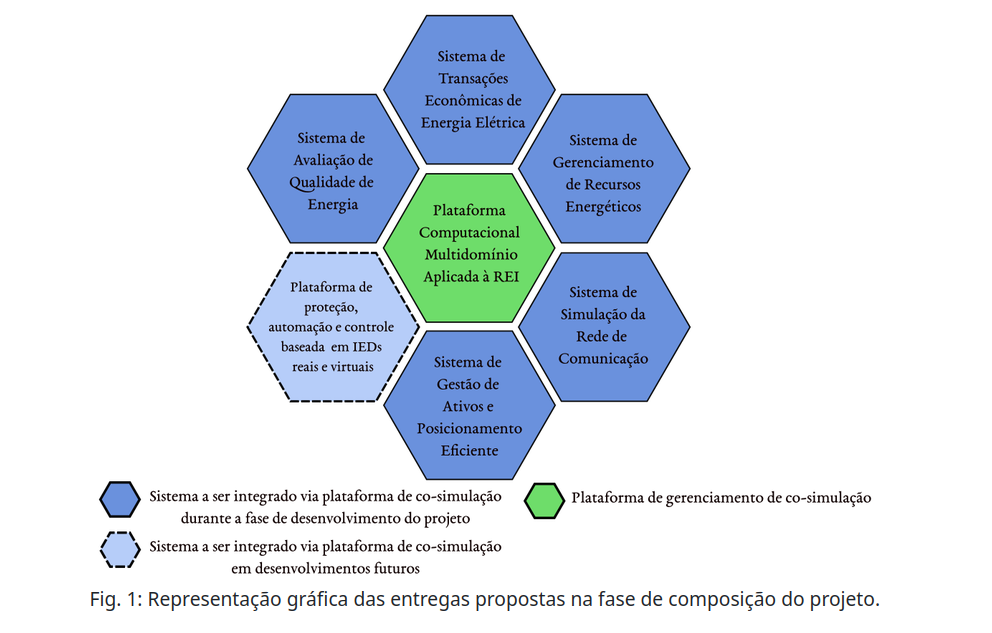
\includegraphics[width=0.62\columnwidth]{figures/opentes_ecosistema.png}
    \caption{Arquitetura multidomínio proposta no projeto OpenTES, integrando quatro frentes especializadas.}
    \label{fig:opentes_eco}
\end{figure}

\begin{itemize}
    \item \textbf{Time de Modelagem e Simulação de Transações Econômicas e Otimização de Prosumidores (TTESO):} atua na formulação matemática e implementação de modelos de mercado transativo de energia e algoritmos de otimização em ambiente de co-simulação;
    \item \textbf{Time de Modelagem e Simulação da Rede Elétrica (TSRE):} responsável pela modelagem elétrica, cálculo de fluxo de potência e validação de redes de distribuição com recursos energéticos distribuídos;
    \item \textbf{Time de Análise da Qualidade de Energia Elétrica e Análise de Dados de Simulação (TSDQ):} desenvolve interfaces analíticas, padronização de metadados e indicadores para avaliação da qualidade de energia e visualização dos dados gerados;
    \item \textbf{Time de Simulação de Comunicação e Co-simulação (TSCC):} responsável pela modelagem da infraestrutura de rede de comunicação, pelo sincronismo entre simuladores heterogêneos e pela replicabilidade conteinerizada da arquitetura.
\end{itemize}

O presente artigo documenta a ferramenta desenvolvida pelo time TSCC, disponibilizada publicamente em código aberto no repositório \texttt{grei-ufc/tscc-com-opentes}~\cite{tscc_repo}.

% ==========================================================================
% 2. INTRODUÇÃO
% ==========================================================================
\section{Introdução}

O projeto OpenTES visa consolidar um espaço de simulação multidomínio para redes elétricas inteligentes (\textit{Smart Grids}) no qual a tomada de decisão dos agentes interaja diretamente com a dinâmica física e elétrica do sistema. Na operação real de redes elétricas modernas, a infraestrutura de telecomunicações desempenha um papel que transcende a simples transferência de dados, atuando como parte integrante da malha de controle distribuído e de coordenação de mercados transativos.

Algoritmos de consenso, recomposição automática de alimentadores e leilões de energia P2P dependem de condições temporais determinísticas. Uma latência imprevista, uma rajada de perda de pacotes ou o transbordamento de fila (\textit{buffer overflow}) em um enlace de baixa capacidade podem atrasar um comando de proteção ou invalidar lances em um mercado energético. Apesar disso, a maioria das simulações de Sistemas Multiagentes (SMA) adota a hipótese simplificadora de comunicação ideal — assumindo entrega instantânea, banda infinita e perda nula.

Para superar essa limitação e transformar a rede de comunicação em uma variável experimental controlável, este trabalho apresenta uma arquitetura de co-simulação tripla que integra três tecnologias complementares:

\begin{enumerate}
    \item \textbf{Python Agent Development Framework (PADE):} proposto por Melo et al.~\cite{melo2019pade}, o PADE é um framework orientado ao desenvolvimento de sistemas multiagentes aplicados a sistemas elétricos de potência, construído sobre a biblioteca assíncrona \textit{Twisted}. O PADE implementa nativamente os padrões da \textit{Foundation for Intelligent Physical Agents} (FIPA), incluindo a estrutura de mensagens FIPA-ACL (\textit{Agent Communication Language})~\cite{fipa2002acl} e protocolos padronizados de requisição e subscrição, conferindo autonomia e inteligência decisória aos agentes;
    \item \textbf{OMNeT++ (\textit{Objective Modular Network Testbed in C++}):} desenvolvido por Varga~\cite{varga2010omnetpp}, trata-se de um simulador modular de eventos discretos em C++ amplamente empregado para modelagem de redes de telecomunicações. No arcabouço proposto, o OMNeT++ modela os enlaces físicos (\texttt{cDatarateChannel}), filas de transmissão por porta (\texttt{cPacketQueue}), taxas de erro de pacote (PER), atrasos de propagação espacial e jitter estocástico;
    \item \textbf{Mosaik:} concebido por Steinbrink et al.~\cite{steinbrink2019mosaik} para testes de sistemas de energia ciberfísicos (CPES), o Mosaik atua como orquestrador mestre da co-simulação. Ele gerencia o grafo de fluxo de dados entre simuladores heterogêneos, coordena o avanço discreto do tempo (\textit{step-by-step}) e resolve dependências cíclicas entre agentes e rede por meio de conexões deslocadas no tempo (\texttt{time\_shifted}).
\end{enumerate}

A fusão desses três pacotes de software, interligados por sockets ZeroMQ~\cite{hintjens2013zeromq} e encapsulados em containers Docker, estabelece uma ferramenta reproduzível na qual o pesquisador configura a topologia, a quantidade de agentes e as tecnologias de enlace sem alterar uma única linha do código de negócio FIPA-ACL dos agentes.

% ==========================================================================
% 3. TRABALHOS CORRELATOS E COMPARAÇÃO DE FERRAMENTAS
% ==========================================================================
\section{Trabalhos Correlatos e Comparação de Ferramentas}

A integração entre simuladores de sistemas de potência, plataformas multiagentes e simuladores de redes de comunicação tem na família de ferramentas \textbf{COSIMA} (\textit{Communication Simulation with Mosaik})~\cite{prost2021cosima} e em sua extensão \textbf{cosima-mango}~\cite{schrage2023cosimamango} suas principais referências na literatura recente. O COSIMA acopla o Mosaik ao OMNeT++/INET para avaliar o tráfego de comunicação em cenários de redes inteligentes, enquanto o \textit{cosima-mango} investiga a robustez de sistemas multiagentes baseados no framework Python \textbf{Mango}.

A Tabela~\ref{tab:pade_mango} sintetiza a comparação estrutural entre o PADE (adotado neste trabalho) e o Mango (utilizado no \textit{cosima-mango}). O PADE destaca-se no contexto de sistemas elétricos por oferecer conformidade nativa com o padrão FIPA-ACL e um driver oficial integrado à API 3.0 do Mosaik (\texttt{MosaikCon}), ao passo que o Mango exige a implementação manual de adaptadores de sincronização e estruturas de mensagens pelo usuário.

\begin{table}[H]
\centering
\caption{Comparação estrutural entre os frameworks multiagentes PADE e Mango.}
\label{tab:pade_mango}
\footnotesize
\begin{tabularx}{\columnwidth}{@{}lXX@{}}
\toprule
\textbf{Critério} & \textbf{PADE~\cite{melo2019pade}} & \textbf{Mango~\cite{schrage2023cosimamango}} \\
\midrule
Domínio-alvo & Redes elétricas inteligentes & Propósito geral \\
Padrão FIPA-ACL & Nativo (\texttt{ACLMessage}, \texttt{AID}) & A cargo do usuário \\
Motor assíncrono & \textit{Twisted} (orientado a eventos) & \texttt{asyncio} \\
Driver Mosaik & Nativo (\texttt{MosaikCon}, API 3.0) & \textit{Wrappers} manuais \\
Telemetria nativa & Registro estruturado em CSV & A cargo do usuário \\
\bottomrule
\end{tabularx}
\end{table}

Adicionalmente, a análise técnica do COSIMA revelou lacunas importantes de usabilidade e engenharia que motivaram a construção do \texttt{tscc-com-opentes}: o COSIMA apresenta acoplamento complexo dependente de configurações estáticas de cenários OMNeT++, não disponibiliza geração paramétrica automática de múltiplas topologias (estrela, malha e anel) via interface gráfica ou CLI, e carece de uma arquitetura de containers pronta para execução imediata em ambientes de nuvem. A Tabela~\ref{tab:comp_ferramentas} compara diretamente a ferramenta desenvolvida neste trabalho com o COSIMA e com simulações PADE convencionais.

\begin{table}[H]
\centering
\caption{Comparação funcional entre o PADE isolado, o COSIMA e a ferramenta proposta (\texttt{tscc-com-opentes}).}
\label{tab:comp_ferramentas}
\scriptsize
\begin{tabularx}{\columnwidth}{@{}lXXX@{}}
\toprule
\textbf{Recurso / Característica} & \textbf{PADE Isolado} & \textbf{COSIMA~\cite{prost2021cosima}} & \textbf{TSCC-OpenTES (Proposto)} \\
\midrule
Camada física de rede & Ideal (TCP local sem perdas) & OMNeT++ / INET & OMNeT++ 6.0 (\texttt{AgentNode}) \\
Transporte Mosaik--Rede & Não aplicável & Protobuf / Sockets customizados & ZeroMQ \texttt{REQ/REP} (\textit{lock-step}) \\
Geração de topologia \texttt{.ned} & Não possui & Estática / manual & Dinâmica em runtime (\texttt{scenario.py}) \\
Topologias nativas & Arbitrária (sem física) & Cenários fixos & Estrela, Malha e Anel ($N$ até 500) \\
Perfis de enlace prontos & Não possui & Configurados manualmente & Cabeada, 5G, Wireless, 4G e 2G \\
Transparência FIPA-ACL & Nativa & Requer adaptação de payload & Interceptação transparente de \texttt{send()} \\
Conteinerização Docker & Não nativo & Parcial / complexa & 3 containers (\texttt{service:pade}) \\
Interfaces de uso & Código Python & Scripts de configuração & Web (Streamlit) + CLI (\texttt{menu.py}) \\
\bottomrule
\end{tabularx}
\end{table}

% ==========================================================================
% 4. ARQUITETURA E DESENVOLVIMENTO DA FERRAMENTA
% ==========================================================================
\section{Arquitetura e Desenvolvimento da Ferramenta}

\subsection{Visão Geral e Fluxo de Co-Simulação}

A arquitetura do \texttt{tscc-com-opentes} é composta por três containers Docker (\texttt{pade}, \texttt{mosaik\_master} e \texttt{omnet\_sim}) que compartilham o mesmo namespace de rede Linux (\texttt{network\_mode: "service:pade"}), comunicando-se via interface de \textit{loopback} (\texttt{127.0.0.1}). Essa decisão de engenharia elimina bloqueios de roteamento entre bridges Docker em ambientes virtualizados ou em nuvem, como o GitHub Codespaces, mantendo o isolamento de processos e dependências de cada tecnologia. A Figura~\ref{fig:arquitetura_tikz} apresenta o diagrama vetorial da arquitetura e o fluxo de dados em cada passo de simulação.

\begin{figure}[H]
\centering
\resizebox{\columnwidth}{!}{%
\begin{tikzpicture}[
    node distance=0.8cm and 0.9cm,
    box/.style={rectangle, rounded corners=4pt, draw=codegreen!90!black, line width=0.9pt, fill=codebg, align=center, font=\sffamily\scriptsize, minimum height=1.25cm, inner sep=5pt},
    subbox/.style={rectangle, rounded corners=2pt, draw=black!50, fill=white, align=center, font=\sffamily\tiny, inner sep=3pt},
    arrow/.style={-{Stealth[length=2.2mm,width=1.6mm]}, line width=0.8pt, draw=codegreen!90!black},
    dashedarrow/.style={-{Stealth[length=2.0mm,width=1.5mm]}, line width=0.7pt, dashed, draw=codeblue!80!black}
]

% Container PADE
\node[box, minimum width=2.4cm] (pade) {
    \textbf{Container \texttt{pade}}\\
    Agentes FIPA-ACL\\
    (\texttt{pade\_star/malha/anel})\\
    \texttt{:5678} (Twisted)
};

% Container MOSAIK
\node[box, right=1.15cm of pade, minimum width=2.6cm] (mosaik) {
    \textbf{Container \texttt{mosaik\_master}}\\
    \texttt{scenario.py} (Orquestrador)\\
    \texttt{omnet\_wrapper.py}\\
    \texttt{collector.py}
};

% Container OMNET
\node[box, right=1.15cm of mosaik, minimum width=2.5cm] (omnet) {
    \textbf{Container \texttt{omnet\_sim}}\\
    OMNeT++ 6.0 (C++17)\\
    \texttt{MosaikBridge.cc (:5555)}\\
    \texttt{AgentNode.cc} + Filas
};

% Artefatos inferiores
\node[subbox, below=0.75cm of mosaik, minimum width=3.6cm] (artefatos) {
    \textbf{Artefatos Gerados e Telemetria}\\
    \texttt{DynamicNetwork.ned} $\cdot$ \texttt{posicoes/links.json}\\
    \texttt{results.csv} $\cdot$ Dashboards \texttt{grafico\_*.png}
};

% Interfaces superiores
\node[subbox, above=0.65cm of mosaik, minimum width=4.2cm] (ui) {
    \textbf{Camada de Configuração do Usuário}\\
    CLI (\texttt{menu.py}) $\cdot$ Web UI (\texttt{menu-streamlit.py})\\
    \texttt{TOPOLOGY}, \texttt{NUM\_PERIFERICOS}, \texttt{TIPOS\_REDE}, \texttt{RANDOM\_SEED}
};

% Setas PADE <-> MOSAIK
\draw[arrow] ([yshift=6pt]pade.east) -- node[above, font=\sffamily\tiny] {\texttt{val\_out} (JSON)} ([yshift=6pt]mosaik.west);
\draw[arrow] ([yshift=-6pt]mosaik.west) -- node[below, font=\sffamily\tiny] {\texttt{val\_in} (\texttt{t+1})} ([yshift=-6pt]pade.east);

% Setas MOSAIK <-> OMNET
\draw[arrow] ([yshift=6pt]mosaik.east) -- node[above, font=\sffamily\tiny] {ZMQ \texttt{REQ} (\texttt{STEP})} ([yshift=6pt]omnet.west);
\draw[arrow] ([yshift=-6pt]omnet.west) -- node[below, font=\sffamily\tiny] {ZMQ \texttt{REP} (\texttt{ACK})} ([yshift=-6pt]mosaik.east);

% Setas UI e Artefatos
\draw[dashedarrow] (ui.south) -- (mosaik.north);
\draw[dashedarrow] (ui.south -| pade.north) -- (pade.north);
\draw[dashedarrow] (mosaik.south) -- (artefatos.north);
\draw[dashedarrow] (artefatos.east) -| node[pos=0.25, below, font=\sffamily\tiny] {\texttt{.ned}} (omnet.south);

\end{tikzpicture}%
}
\caption{Fluxograma da arquitetura de co-simulação tripla do \texttt{tscc-com-opentes} e troca de mensagens entre containers.}
\label{fig:arquitetura_tikz}
\end{figure}

\subsection{Interceptação Transparente FIPA-ACL no PADE}

Para que os agentes PADE utilizem suas primitivas nativas (\texttt{self.send(msg)} e \texttt{self.react(msg)}) sem que as mensagens trafeguem diretamente por sockets TCP do sistema operacional (o que contornaria a simulação de rede física), foi implementado um **interceptador de plano de dados** nas classes de agentes (\texttt{AgenteFIPA}, \texttt{AgenteMalhaFIPA} e \texttt{AgenteAnelFIPA}).

Quando um agente executa \texttt{self.send(message)}, o método verifica o atributo \texttt{ontology} da mensagem FIPA-ACL:
\begin{itemize}
    \item \textbf{Plano de Dados (Simulação):} se a ontologia corresponder ao tráfego da co-simulação (\texttt{telemetria\_rede} na estrela/malha ou \texttt{malha\_restrita} no anel), o objeto \texttt{ACLMessage} é serializado em uma string JSON contendo \texttt{performative}, \texttt{sender}, \texttt{receivers}, \texttt{content}, \texttt{ontology} e \texttt{conversation\_id}. Caso o agente envie múltiplas mensagens no mesmo passo discreto, os objetos JSON são concatenados de forma síncrona no buffer de saída \texttt{self.val\_out} utilizando o delimitador \texttt{|||}, prevenindo a sobrescrita de pacotes em rajadas;
    \item \textbf{Plano de Controle:} mensagens internas do sistema PADE seguem o fluxo padrão da superclasse \texttt{Agent}.
\end{itemize}

Na direção oposta, durante o método \texttt{step(time, inputs)} do driver \texttt{MosaikSim}, as strings recebidas na porta \texttt{val\_in} são desmultiplexadas por \texttt{split("|||")}, reconstruídas em instâncias \texttt{ACLMessage} via \texttt{json\_to\_acl()} e entregues diretamente ao método \texttt{self.react(msg)} de cada agente destinatário.

\subsection{Sincronismo Lock-Step via ZeroMQ e Geração Dinâmica de Topologia}

O orquestrador \texttt{scenario.py} constrói programaticamente a topologia antes de iniciar os simuladores:
\begin{enumerate}
    \item Lê as variáveis de ambiente \texttt{TOPOLOGY}, \texttt{NUM\_PERIFERICOS}, \texttt{TIPOS\_REDE}, \texttt{RANDOM\_SEED} e \texttt{SIM\_STEPS};
    \item Calcula as coordenadas cartesianas $(x, y) \in [0, 1000]\times[0, 1000]\text{ m}$ de cada agente e gera a lista de enlaces associando ciclicamente os perfis tecnológicos selecionados;
    \item Persiste os metadados da rodada em \texttt{posicoes.json}, \texttt{links.json} e \texttt{config.json} e escreve atomicamente o arquivo de topologia \texttt{DynamicNetwork.ned};
    \item Conecta cada entidade \texttt{PadeAgent} ao seu respectivo \texttt{AgentNode} no OMNeT++ no sentido de envio (\texttt{val\_out} $\to$ \texttt{val\_in}) e, no sentido de retorno, utiliza \texttt{time\_shifted=True} com \texttt{initial\_data=\{'val\_out': ''\}} para quebrar o laço algébrico de causalidade entre os dois simuladores do tipo \texttt{time-based}.
\end{enumerate}

O acoplamento entre o adaptador Python (\texttt{omnet\_wrapper.py}) e o motor C++ do OMNeT++ (\texttt{MosaikBridge.cc}) opera em regime \textit{lock-step} sobre um par de sockets ZeroMQ \texttt{REQ/REP} na porta TCP \texttt{5555}. A cada passo $t$, o \texttt{OmnetAdapter} envia um payload JSON \texttt{STEP} contendo o tempo $t$, os inputs dos nós e a resolução temporal (\texttt{time\_resolution = 1.0\text{ s}}). O \texttt{MosaikBridge} bloqueia a execução enquanto injeta os payloads nos módulos \texttt{AgentNode}, agenda um evento discreto para $t_{\text{sim}} + \Delta t$ (\texttt{scheduleAt(simTime() + timeResolution)}) e, ao atingir o próximo passo, coleta as métricas e mensagens entregues em todos os nós, devolvendo o pacote JSON de confirmação com o contador \texttt{mosaik\_step}.

\subsection{Modelagem Física de Canais e Filas no OMNeT++}

Os cinco perfis tecnológicos de canal são declarados em \texttt{Profiles.ned} como especializações de \texttt{ned.DatarateChannel}, cujos parâmetros físicos de taxa de transmissão ($R$), atraso base ($d_{\text{canal}}$) e taxa de erro de pacote (PER) estão resumidos na Tabela~\ref{tab:perfis_enlace}.

\begin{table}[H]
\centering
\caption{Parâmetros físicos dos perfis de enlace em \texttt{Profiles.ned}.}
\label{tab:perfis_enlace}
\footnotesize
\begin{tabularx}{\columnwidth}{@{}lXll@{}}
\toprule
\textbf{Perfil NED} & \textbf{Taxa ($R$)} & \textbf{Atraso Base ($d_{\text{canal}}$)} & \textbf{PER} \\
\midrule
\texttt{Link\_Wired} & $1\text{ Gbps}$ & $1\text{ ms}$ (fixo) & $0\%$ \\
\texttt{Link\_5G} & $500\text{ Mbps}$ & $\text{truncnormal}(5\text{ ms}, 1\text{ ms})$ & $0{,}001\%$ \\
\texttt{Link\_Wireless} & $300\text{ Mbps}$ & $\text{truncnormal}(2\text{ ms}, 0{,}5\text{ ms})$ & $0{,}1\%$ \\
\texttt{Link\_4G} & $50\text{ Mbps}$ & $\text{truncnormal}(35\text{ ms}, 8\text{ ms})$ & $0{,}5\%$ \\
\texttt{Link\_2G} & $250\text{ kbps}$ & $\text{exponential}(200\text{ ms})$ & $15\%$ \\
\bottomrule
\end{tabularx}
\end{table}

Sobre esses canais, o módulo C++ \texttt{AgentNode.cc} implementa quatro mecanismos físicos:
\begin{enumerate}
    \item \textbf{Roteamento Seletivo por Destinatário:} ao receber uma string JSON em \texttt{val\_in}, o nó analisa o array \texttt{receivers} com a biblioteca \texttt{nlohmann/json} e encaminha o pacote \texttt{AgentPacket} exclusivamente pelas portas de saída conectadas aos destinatários especificados;
    \item \textbf{Fila Finita de Transmissão e \textit{Buffer Overflow}:} cada porta de saída $k$ possui uma fila \texttt{cPacketQueue} com capacidade máxima de 5 pacotes. Se o canal estiver ocupado (\texttt{txChannel->isBusy()}) e $\text{len}(\text{queue}_k) \ge 5$, o pacote excedente é descartado na origem e incrementado em \texttt{packets\_dropped};
    \item \textbf{Atraso Espacial e Jitter Dinâmico:} na inicialização, calcula-se a distância euclidiana $d = \sqrt{(x_i - x_j)^2 + (y_i - y_j)^2}$ entre nós conectados, adicionando o atraso de propagação espacial de $50\,\mu\text{s/m}$ ao atraso do canal (\texttt{cDatarateChannel} ou \texttt{cDelayChannel}). A cada pacote transmitido em canais cujo atraso-base supera $1{,}5\text{ ms}$, aplica-se uma perturbação estocástica uniforme $\eta \in [-0{,}25\,d_{\text{base}},\, +0{,}25\,d_{\text{base}}]$, resultando na latência fim a fim $L$:
    \begin{equation}
        L = d_{\text{canal}} + \frac{8S}{R} + 5\times 10^{-5}\,d + \eta
        \label{eq:latencia}
    \end{equation}
    onde $S$ é o tamanho do pacote em bytes;
    \item \textbf{Descarte por PER do Canal e Atenuação por Distância:} na chegada ao receptor (\texttt{handleMessage}), o pacote é descartado se o canal físico sinalizar erro de bit (\texttt{pkt->hasBitError()}, governado pelo PER da Tabela~\ref{tab:perfis_enlace}) ou segundo a probabilidade de atenuação espacial e tamanho de pacote $P_{\text{drop,dist}}$:
    \begin{equation}
        P_{\text{drop,dist}} = \min\!\left(0{,}99;\; \frac{d}{100}\cdot 0{,}015\cdot \max\!\left(1;\; \frac{S}{15000}\right)\right)
        \label{eq:drop}
    \end{equation}
\end{enumerate}

% ==========================================================================
% 5. GUIA DE USO E OPERAÇÃO DA PLATAFORMA
% ==========================================================================
\section{Guia de Uso e Operação da Plataforma}

A ferramenta foi projetada para que pesquisadores e estudantes possam configurar, executar e analisar cenários de co-simulação de forma imediata, sem necessidade de compilar manualmente o OMNeT++ ou editar arquivos C++ e NED.

\subsection{Pré-requisitos e Instalação}

O único requisito para execução completa é possuir o \textbf{Docker} e o \textbf{Docker Compose} instalados (localmente ou em ambiente GitHub Codespaces), além de Python 3.10+ para os menus de inicialização. Obtém-se o repositório com:

\begin{lstlisting}[style=shellstyle]
git clone -b development https://github.com/grei-ufc/tscc-com-opentes.git
cd tscc-com-opentes
\end{lstlisting}

\subsection{Modos de Operação: CLI e Interface Web}

O usuário dispõe de três formas equivalentes para parametrizar e iniciar uma co-simulação:

\paragraph{1. Configurador Interativo via Terminal (CLI):} ideal para servidores remotos, SSH ou GitHub Codespaces. Ao executar \texttt{python3 menu.py}, o usuário é guiado em três etapas interativas:
\begin{lstlisting}[style=shellstyle]
$ python3 menu.py
1. TOPOLOGIA DE REDE: [1] Estrela | [2] Malha | [3] Anel
Escolha [1/2/3]: 1
2. NUMERO DE AGENTES PERIFERICOS [1-500]: 20
3. TECNOLOGIAS DE ENLACE:
   [1] Cabeada | [2] 5G | [3] Wireless | [4] 4G | [5] 2G
Tecnologias [1-5 ou ENTER para todas]:
Iniciar simulacao? [s/n]: s
\end{lstlisting}

\paragraph{2. Interface Gráfica Web (Streamlit):} iniciada com \texttt{streamlit run menu-streamlit.py}. Oferece pré-visualização interativa do grafo da topologia (Plotly), seleção individual de tecnologia de enlace por agente na estrela e no anel, terminal embutido com transmissão de logs em tempo real e aba dedicada para inspeção imediata dos dashboards gerados ao término da rodada.

\paragraph{3. Execução Direta via Variáveis de Ambiente:} para automação de lotes experimentais (\textit{batch runs}) e reprodutibilidade científica com semente fixa:
\begin{lstlisting}[style=shellstyle]
TOPOLOGY=estrela NUM_PERIFERICOS=20 \
TIPOS_REDE=Link_Wired,Link_5G,Link_4G,Link_2G,Link_Wireless \
RANDOM_SEED=42 SIM_STEPS=20 \
docker compose up --build --force-recreate \
  --abort-on-container-exit --exit-code-from mosaik_master
\end{lstlisting}

A Tabela~\ref{tab:semantica_topologias} resume como o parâmetro \texttt{NUM\_PERIFERICOS} ($N$) define a escala e o padrão de tráfego em cada topologia suportada.

\begin{table}[H]
\centering
\caption{Semântica do parâmetro $N$ (\texttt{NUM\_PERIFERICOS}) nas três topologias da plataforma.}
\label{tab:semantica_topologias}
\scriptsize
\begin{tabularx}{\columnwidth}{@{}lccp{3.3cm}@{}}
\toprule
\textbf{Topologia} & \textbf{Total de Nós} & \textbf{Enlaces} & \textbf{Padrão de Tráfego por Passo} \\
\midrule
\texttt{estrela} & $1 + N$ & $N$ & Central envia $N$ \texttt{REQUEST}; periféricos respondem \texttt{INFORM} \\
\texttt{malha} & $N$ ($N\ge 2$) & $\frac{N(N-1)}{2}$ & Todos os $N$ agentes enviam \texttt{INFORM} aos $N-1$ pares \\
\texttt{anel} & $N$ ($N\ge 3$) & $N$ & Cada agente envia \texttt{INFORM} aos 2 vizinhos imediatos \\
\bottomrule
\end{tabularx}
\end{table}

\subsection{Artefatos de Saída e Validação Automatizada}

Ao final de cada execução, a ferramenta exporta automaticamente:
\begin{itemize}
    \item \texttt{mosaik-dir/results.csv}: série temporal completa com \texttt{packets\_sent}, \texttt{packets\_received}, \texttt{packets\_dropped}, \texttt{packet\_sizes\_out}, \texttt{latencies\_out}, \texttt{jitters\_out} e payloads FIPA-ACL (\texttt{val\_out}) por nó e por passo;
    \item \texttt{omnet-dir/posicoes.json}, \texttt{links.json} e \texttt{config.json}: registro exato das coordenadas espaciais e dos canais atribuídos a cada enlace;
    \item \texttt{mosaik-dir/grafico\_trafego\_*.png}: painéis analíticos de alta resolução contendo o mapa topológico georreferenciado, balanço cumulativo de pacotes, séries de latência e jitter com percentil 95 (P95), tamanho de pacotes e taxa de entrega (PDR) por nó.
\end{itemize}

Para verificar a integridade do código C++17 e a execução fim a fim das três topologias de forma automatizada, o repositório inclui uma suíte de testes executável com \texttt{pytest tests/test\_validation\_suite.py}.

% ==========================================================================
% 6. VALIDAÇÃO EXPERIMENTAL E RESULTADOS
% ==========================================================================
\section{Validação Experimental e Resultados}

Para demonstrar a capacidade analítica da plataforma, foram conduzidos três estudos de caso determinísticos (\texttt{RANDOM\_SEED=42}, \texttt{SIM\_STEPS=20} passos de $1\text{ s}$) combinando ciclicamente todas as cinco tecnologias de enlace (\texttt{Link\_Wired}, \texttt{Link\_5G}, \texttt{Link\_4G}, \texttt{Link\_2G} e \texttt{Link\_Wireless}):
\begin{enumerate}
    \item \textbf{Topologia Estrela ($N=20$):} 1 agente central e 20 periféricos (21 agentes, 20 enlaces);
    \item \textbf{Topologia Malha Completa ($N=5$):} 5 agentes \textit{peers} totalmente conectados (10 enlaces bidirecionais);
    \item \textbf{Topologia Anel Bidirecional ($N=5$):} 5 agentes \textit{peers} em ciclo fechado (5 enlaces).
\end{enumerate}

A Tabela~\ref{tab:res_tecnologias} apresenta o desempenho desagregado por tecnologia de enlace na topologia Estrela ($N=20$), enquanto a Tabela~\ref{tab:res_topologias} consolida os indicadores globais obtidos nas três topologias. As Figuras~\ref{fig:dash_estrela}, \ref{fig:dash_malha} e \ref{fig:dash_anel} exibem os dashboards gerados automaticamente pela ferramenta.

\begin{table}[H]
\centering
\caption{Desempenho por tecnologia de enlace na topologia Estrela ($N=20$, 20 passos, \texttt{RANDOM\_SEED=42}).}
\label{tab:res_tecnologias}
\footnotesize
\begin{tabularx}{\columnwidth}{@{}Xrrrr@{}}
\toprule
\textbf{Tecnologia} & \textbf{Lat. Média} & \textbf{Jitter Médio} & \textbf{PDR} & \textbf{Amostras} \\
\midrule
Cabeada & $20{,}1\text{ ms}$ & $0{,}0\,\mu\text{s}$ & $100{,}0\%$ & $156$ \\
Wireless & $23{,}9\text{ ms}$ & $659{,}9\,\mu\text{s}$ & $96{,}5\%$ & $136$ \\
5G & $26{,}8\text{ ms}$ & $1.209{,}2\,\mu\text{s}$ & $98{,}0\%$ & $148$ \\
4G & $48{,}2\text{ ms}$ & $8.952{,}7\,\mu\text{s}$ & $94{,}6\%$ & $139$ \\
2G & $223{,}5\text{ ms}$ & $161.078{,}2\,\mu\text{s}$ & $84{,}7\%$ & $105$ \\
\midrule
\textbf{Global} & $\mathbf{59{,}24\text{ \textbf{ms}}}$ & $\mathbf{26.939{,}1\,\mu\text{\textbf{s}}}$ & $\mathbf{91{,}6\%}$ & $\mathbf{684}$ \\
\bottomrule
\end{tabularx}
\end{table}

\begin{table}[H]
\centering
\caption{Síntese comparativa das três topologias suportadas (20 passos, \texttt{RANDOM\_SEED=42}).}
\label{tab:res_topologias}
\scriptsize
\begin{tabularx}{\columnwidth}{@{}lcccccc@{}}
\toprule
\textbf{Topologia} & \textbf{Nós/Links} & \textbf{Env.} & \textbf{Rec.} & \textbf{Drop} & \textbf{PDR} & \textbf{Lat. Média (P95)} \\
\midrule
Estrela ($N=20$) & $21 / 20$ & $747$ & $684$ & $63$ & $91{,}6\%$ & $59{,}2\text{ ms}$ ($242{,}0\text{ ms}$) \\
Malha ($N=5$) & $5 / 10$ & $400$ & $364$ & $36$ & $91{,}0\%$ & $66{,}8\text{ ms}$ ($279{,}8\text{ ms}$) \\
Anel ($N=5$) & $5 / 5$ & $200$ & $175$ & $25$ & $87{,}5\%$ & $75{,}6\text{ ms}$ ($280{,}4\text{ ms}$) \\
\bottomrule
\end{tabularx}
\end{table}

\begin{figure*}[t]
    \centering
    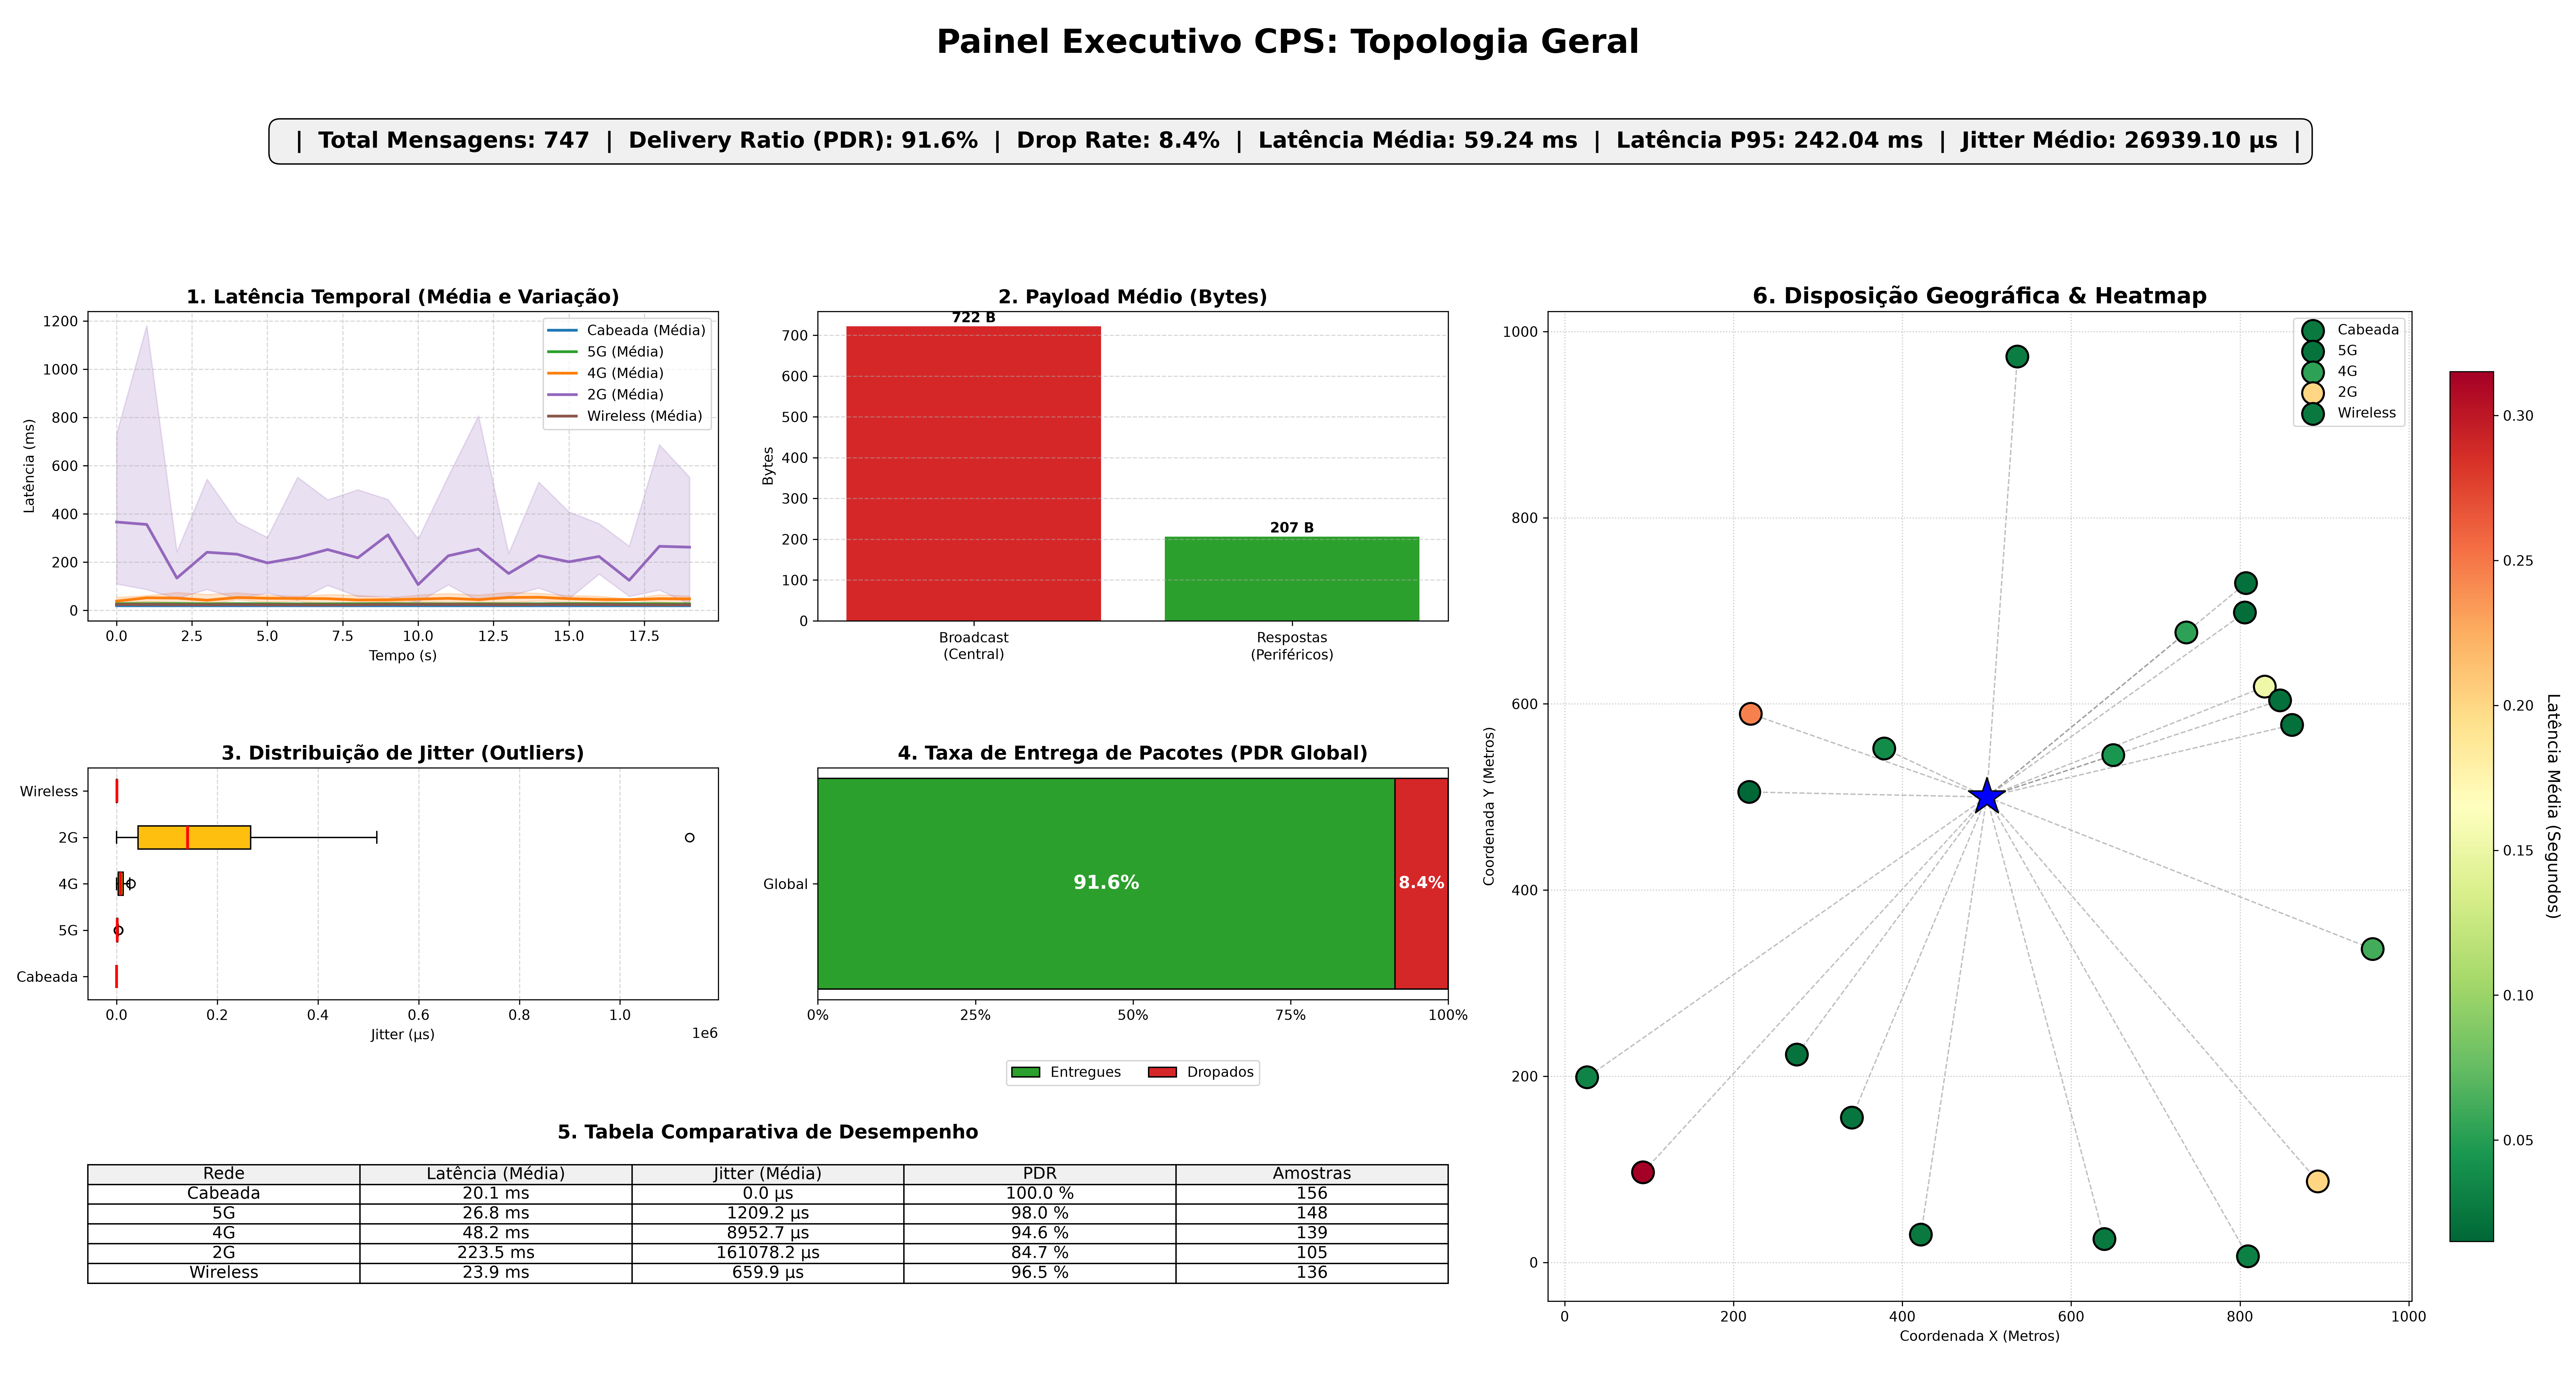
\includegraphics[width=0.92\textwidth]{figures/dashboard_estrela_n20.png}
    \caption{Dashboard consolidado gerado automaticamente pela ferramenta para a topologia Estrela ($1\text{ central} + 20\text{ periféricos} = 21\text{ agentes}$, 20 enlaces, 20 passos; $747$ pacotes enviados, $684$ entregues e $63$ descartados).}
    \label{fig:dash_estrela}
\end{figure*}

\begin{figure}[H]
    \centering
    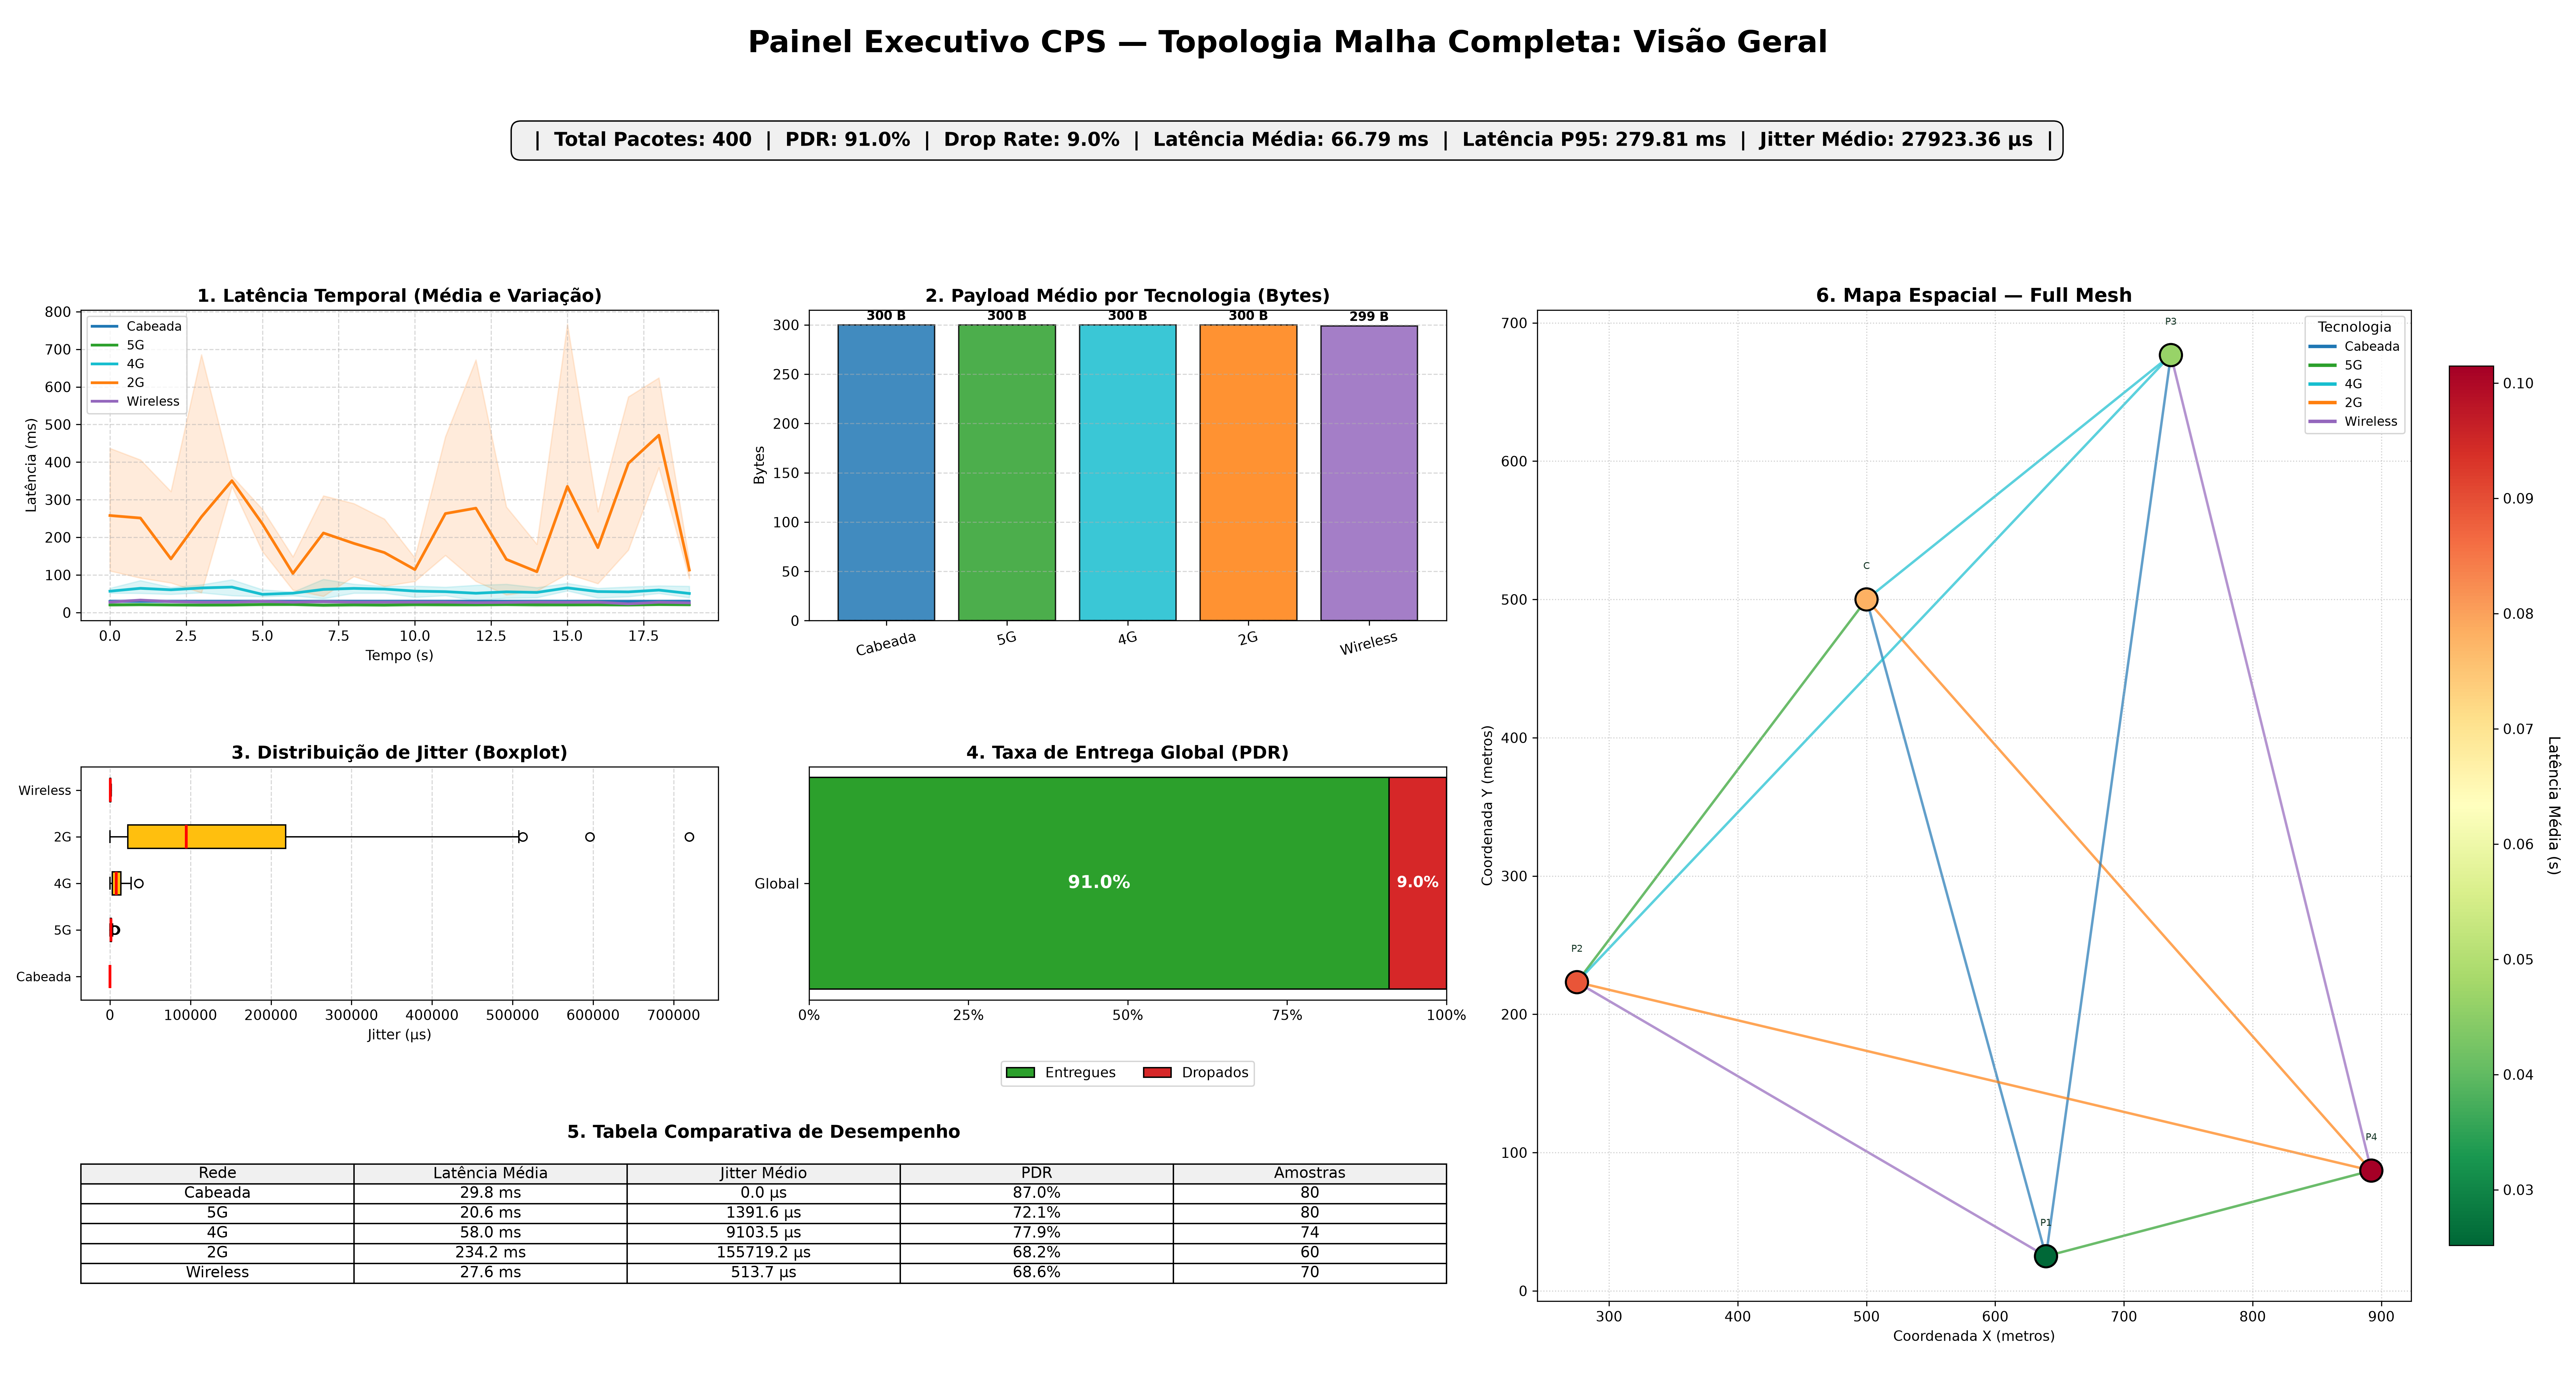
\includegraphics[width=\columnwidth]{figures/dashboard_malha_n5.png}
    \caption{Dashboard consolidado da topologia Malha Completa ($5\text{ agentes peers}$, 10 enlaces, 20 passos; $400$ enviados, $364$ entregues e $36$ descartados).}
    \label{fig:dash_malha}
\end{figure}

\begin{figure}[H]
    \centering
    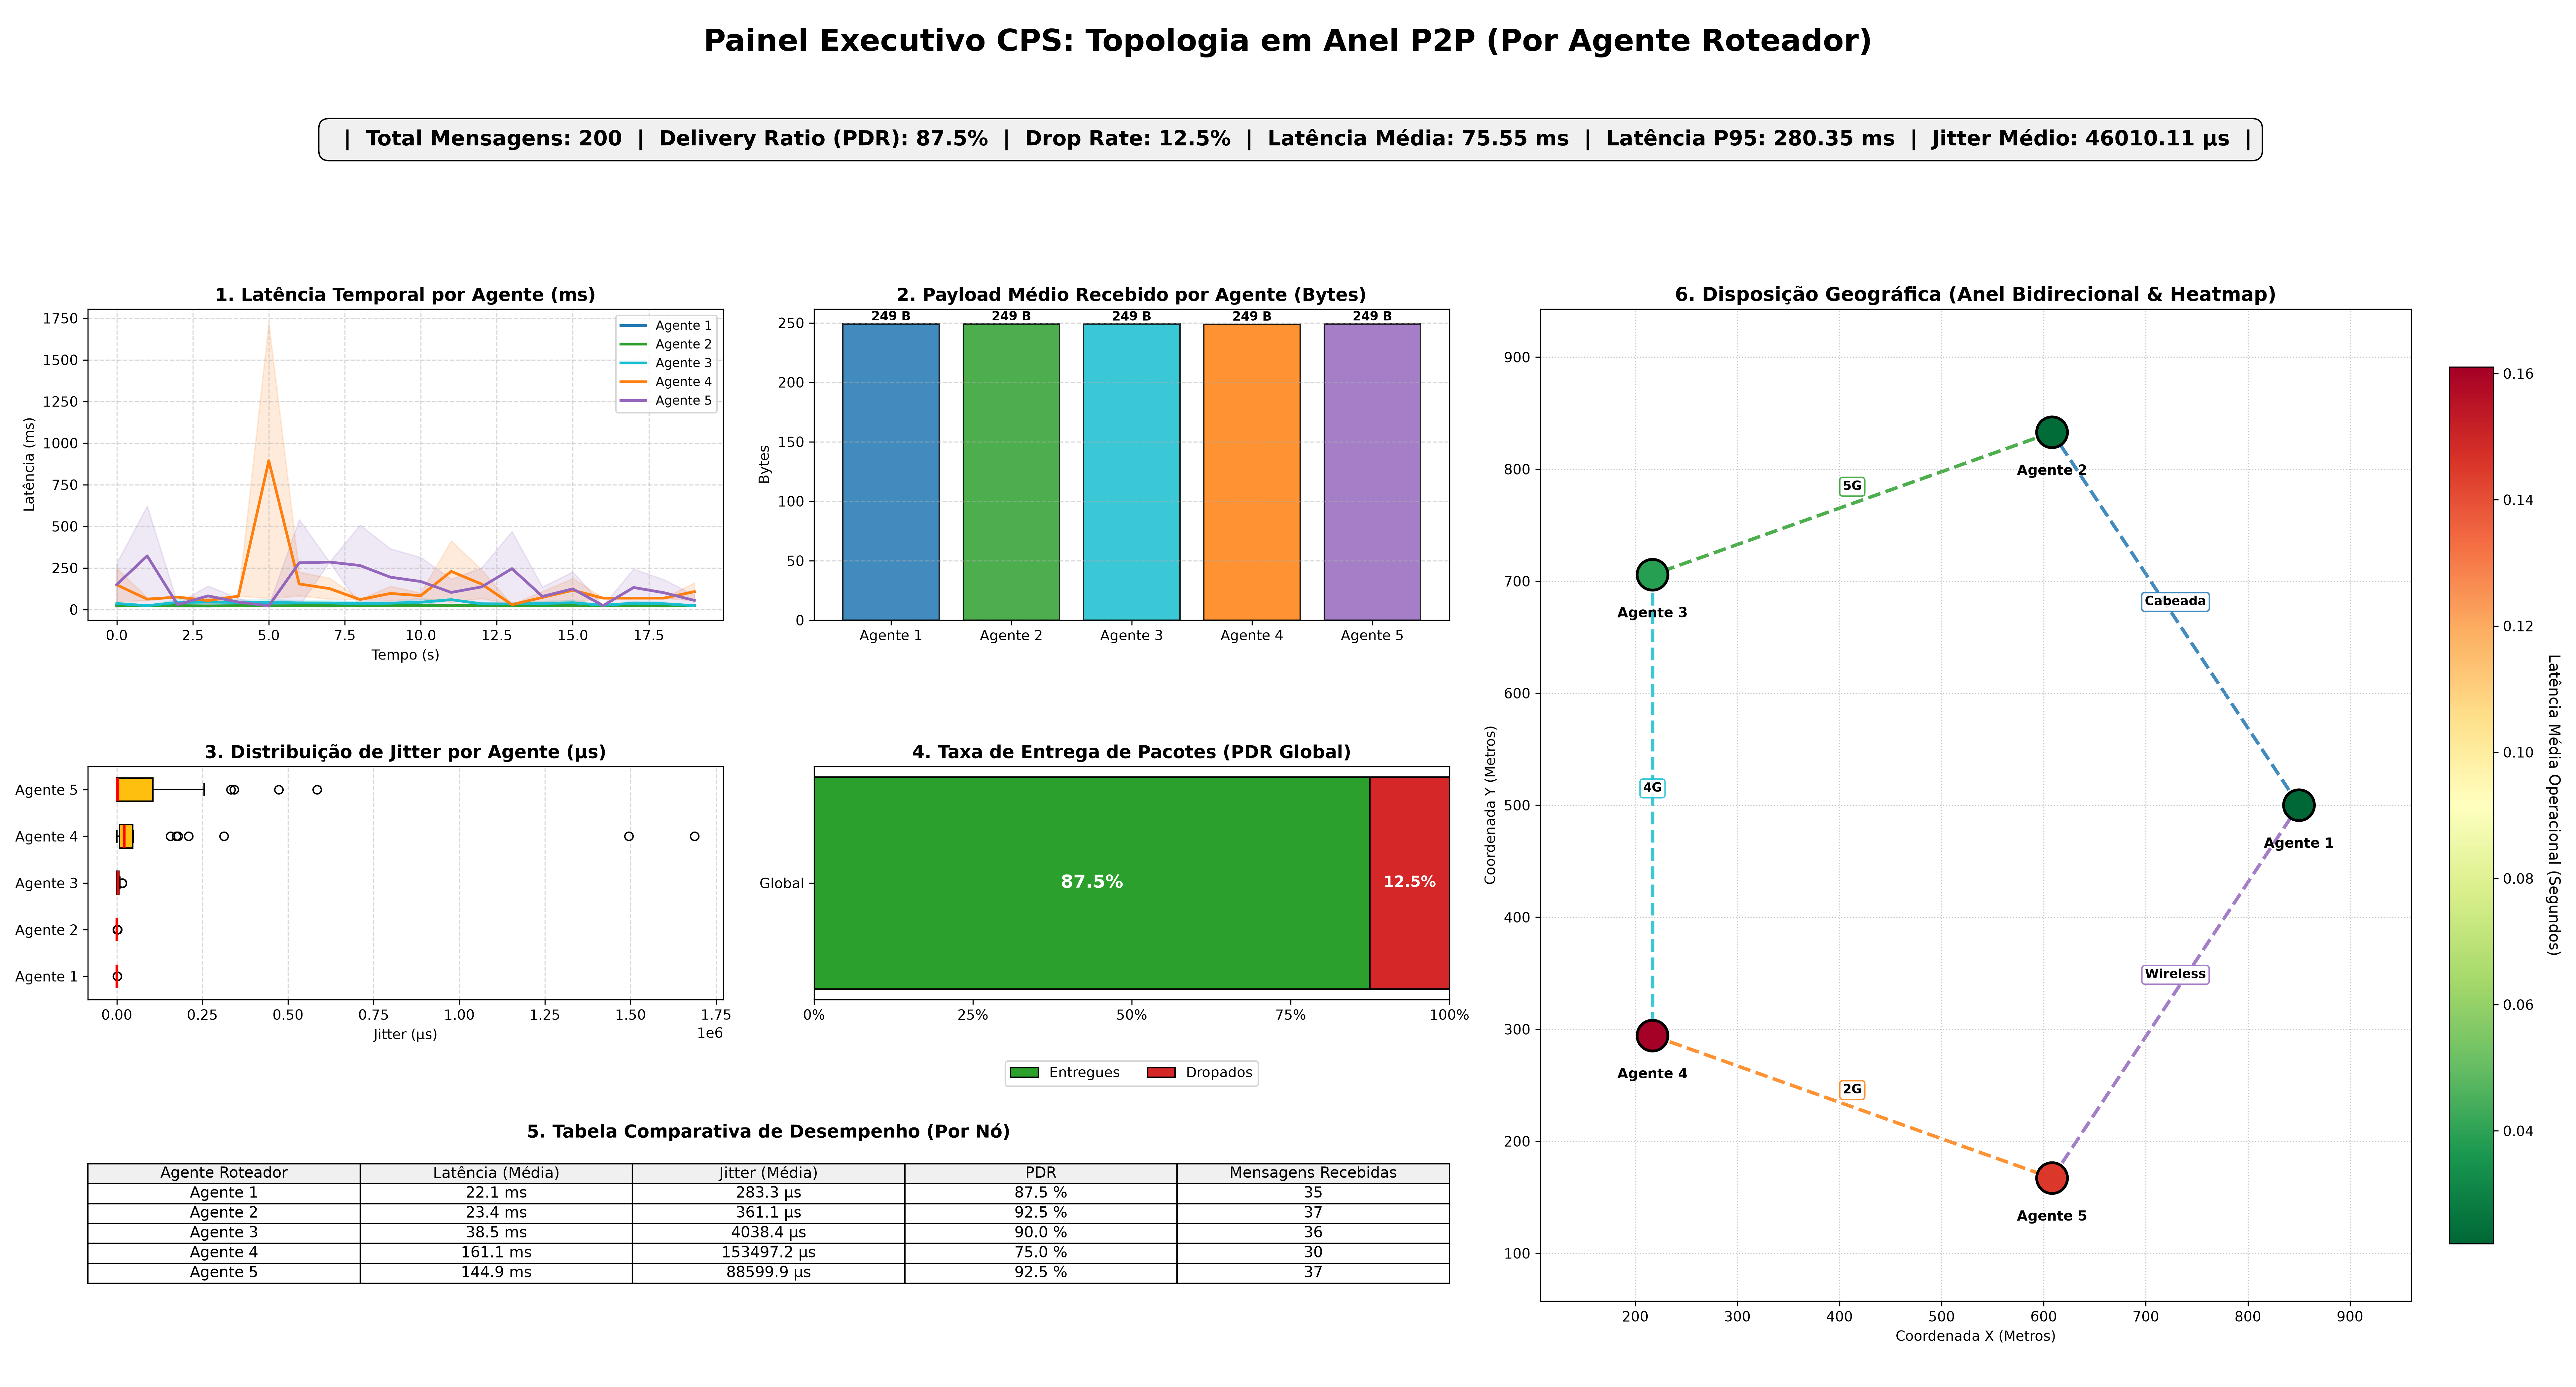
\includegraphics[width=\columnwidth]{figures/dashboard_anel_n5.png}
    \caption{Dashboard consolidado da topologia Anel Bidirecional ($5\text{ agentes peers}$, 5 enlaces em ciclo fechado, 20 passos; $200$ enviados, $175$ entregues e $25$ descartados).}
    \label{fig:dash_anel}
\end{figure}

\subsection{Discussão dos Resultados}

A análise conjunta das Tabelas~\ref{tab:res_tecnologias} e \ref{tab:res_topologias} evidencia três propriedades fundamentais da ferramenta desenvolvida:
\begin{enumerate}
    \item \textbf{Fidelidade física dos canais de comunicação:} na rede \textbf{Cabeada}, a latência média observada é de $20{,}1\text{ ms}$ (soma do atraso base de $1{,}0\text{ ms}$ com o atraso de propagação espacial de $50\,\mu\text{s/m}$ no grid de $1000\times 1000\text{ m}$), com jitter exatamente nulo ($0{,}0\,\mu\text{s}$) e entrega de $100{,}0\%$. Os perfis \textbf{Wireless} e \textbf{5G} apresentam latências baixas ($23{,}9\text{ ms}$ e $26{,}8\text{ ms}$) e alta confiabilidade ($\text{PDR} \ge 96{,}5\%$). O perfil \textbf{4G} opera em patamar intermediário ($48{,}2\text{ ms}$, $\text{PDR} = 94{,}6\%$), enquanto o enlace \textbf{2G} ($250\text{ kbps}$, $\text{PER} = 15\%$) impõe severa degradação ao tráfego dos agentes, elevando a latência média para $223{,}5\text{ ms}$, o jitter médio para $161{,}1\text{ ms}$ e reduzindo a taxa de entrega para $84{,}7\%$;
    \item \textbf{Conservação exata de pacotes em todas as topologias:} em todos os cenários verifica-se a identidade $\text{Enviados} = \text{Recebidos} + \text{Descartados}$ ($747 = 684 + 63$ na estrela; $400 = 364 + 36$ na malha; $200 = 175 + 25$ no anel). Na topologia Estrela, como os periféricos só enviam respostas \texttt{INFORM} quando o \texttt{REQUEST} do nó central chega sem descarte, a perda de pacotes no sentido direto reduz organicamente o número de mensagens de retorno nos passos seguintes;
    \item \textbf{Impacto da topologia sobre o volume de tráfego:} para um mesmo número de agentes ($N=5$), a topologia em Malha Completa demanda o dobro de enlaces físicos ($10$ contra $5$) e gera o dobro de pacotes transmitidos ($400$ contra $200$) em comparação ao Anel Bidirecional, evidenciando o compromisso entre conectividade direta (menor número de saltos) e sobrecarga de mensagens na rede.
\end{enumerate}

% ==========================================================================
% 7. CONCLUSÃO
% ==========================================================================
\section{Conclusão}

Este trabalho apresentou o desenvolvimento, a arquitetura e o modo de operação do \texttt{tscc-com-opentes}, um arcabouço de co-simulação que integra agentes FIPA-ACL no PADE, o simulador de eventos discretos OMNeT++ e o orquestrador Mosaik via ZeroMQ em containers Docker. A ferramenta preenche uma lacuna prática importante em relação a soluções correlatas ao oferecer interceptação transparente de mensagens FIPA-ACL, geração dinâmica em tempo de execução de topologias em estrela, malha completa e anel bidirecional, cinco perfis tecnológicos de enlace prontos para uso e interfaces amigáveis em linha de comando e navegador web.

Os resultados experimentais comprovaram o sincronismo determinístico entre os três simuladores e demonstraram como diferentes infraestruturas de telecomunicações (da fibra cabeada e 5G a enlaces 2G legados) afetam a taxa de entrega, a latência e o jitter das mensagens trocadas pelos agentes. Como trabalhos futuros no escopo do projeto OpenTES, preveem-se o refinamento da resolução temporal para escala sub-segundo, a implementação de fragmentação de pacotes por MTU e o acoplamento direto desta camada de comunicação aos módulos de simulação elétrica (TSRE), mercado transativo (TTESO) e qualidade de energia (TSDQ).

% ==========================================================================
% REFERÊNCIAS BIBLIOGRÁFICAS
% ==========================================================================
\begin{thebibliography}{99}

\bibitem{melo2019pade}
L.~S. Melo, R.~F. Sampaio, R.~P.~S. Leão, G.~C. Barroso, and J.~R. Bezerra, ``Python-based multi-agent platform for application on power grids,'' \textit{International Transactions on Electrical Energy Systems}, vol.~29, no.~6, p.~e12012, 2019. DOI: \texttt{10.1002/2050-7038.12012}.

\bibitem{varga2010omnetpp}
A.~Varga, ``OMNeT++,'' in \textit{Modeling and Tools for Network Simulation}, K.~Wehrle, M.~Güneş, and J.~Gross, Eds. Berlin, Heidelberg: Springer, 2010, pp.~35--59.

\bibitem{steinbrink2019mosaik}
C.~Steinbrink \textit{et al.}, ``CPES Testing with Mosaik: Co-Simulation Planning, Execution and Analysis,'' \textit{Applied Sciences}, vol.~9, no.~5, p.~923, 2019. DOI: \texttt{10.3390/app9050923}.

\bibitem{prost2021cosima}
M.~Prost \textit{et al.}, ``COSIMA: Integration of Communication Simulation into Co-Simulation of Smart Grids with Mosaik,'' OFFIS --- Institute for Information Technology, Oldenburg, Germany, Tech. Rep., 2021. Disponível em: \url{https://cosima.offis.de}.

\bibitem{schrage2023cosimamango}
R.~Schrage \textit{et al.}, ``cosima-mango: Investigating Multi-Agent System robustness through integrated communication simulation,'' OFFIS --- Institute for Information Technology, Oldenburg, Germany, 2023.

\bibitem{fipa2002acl}
FIPA, \textit{FIPA ACL Message Structure Specification}, Standard SC00061G, Foundation for Intelligent Physical Agents, 2002. Disponível em: \url{http://www.fipa.org}.

\bibitem{hintjens2013zeromq}
P.~Hintjens, \textit{ZeroMQ: Messaging for Many Applications}. Sebastopol, CA: O'Reilly Media, 2013.

\bibitem{tscc_repo}
GREI-UFC, ``\texttt{tscc-com-opentes}: Co-simulação PADE + OMNeT++ + Mosaik para Redes Elétricas Inteligentes,'' Grupo de Redes Elétricas Inteligentes, Universidade Federal do Ceará, 2026. Disponível em: \url{https://github.com/grei-ufc/tscc-com-opentes}.

\end{thebibliography}

\end{document}
